\chapter{\ifproject%
\ifenglish Experimentation and Results\else การทดลองและผลลัพธ์\fi
\else%
\ifenglish System Evaluation\else การประเมินระบบ\fi
\fi}

% ในบทนี้จะทดสอบเกี่ยวกับการทำงานในฟังก์ชันหลักๆ
ในบทนี้จะทดสอบระบบการยืนยันตัวตนด้วยการใช้ภาพใบหน้า โดยมีผู้ทดลอง 5 คน 
ทำการทดลองเป็นเวลา 5 วันเพื่อดูผลการทดลองในแต่ละวัน ได้แก่ ความแม่นยำของการระบุตัวตนด้วยใบหน้า 
เวลาในการตรวจจับใบหน้าตลอดถึงการแสดงผล และความพึงพอใจของผู้ทดลองต่อระบบ

\section{ความแม่นยำของการตรวจจับใบหน้า}
การทดสอบนี้จะเป็นการทดสอบเพื่อวัดผลความแม่นยำในการตรวจจับภาพใบหน้า โดยมีรูปภาพใบหน้าบุคคลจำนวน 50 รูป และรูปภาพสัตว์จำนวน 50 รูป 
มาทำการทดลองกับแบบจำลองการตรวจจับใบหน้า จะได้ผลลัพธ์ดังกราฟด้านล่าง

\begin{figure}[!ht]
  \begin{center}
    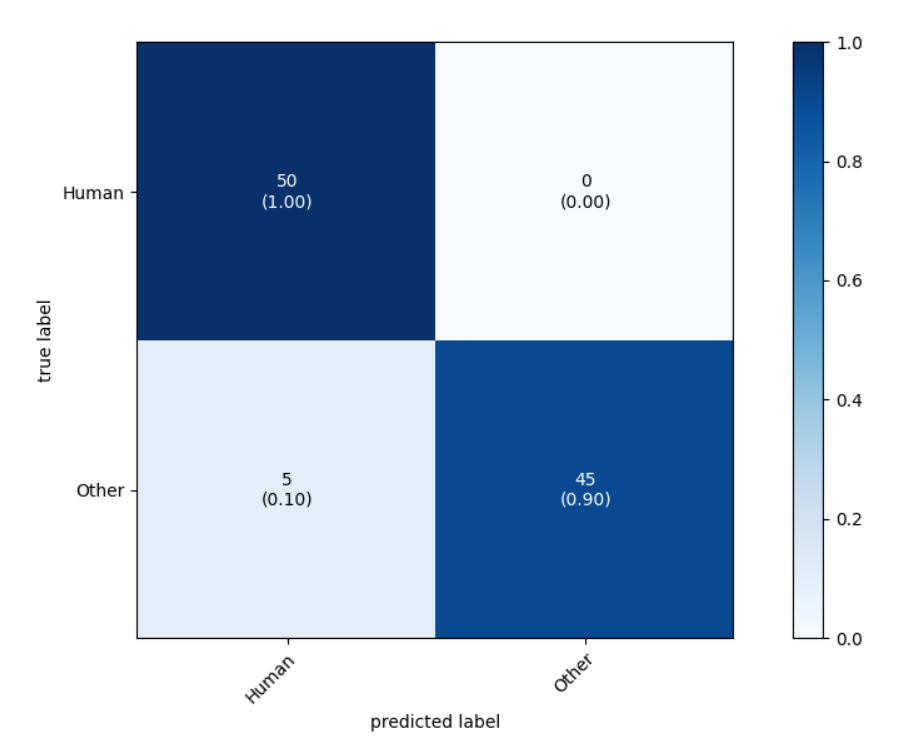
\includegraphics[scale=.45]{pic/face_result.png}
    \caption[กราฟแสดงความแม่นยำของการตรวจจับใบหน้า]{กราฟแสดงความแม่นยำของการตรวจจับใบหน้า}
    \label{fig:acc_graph}
  \end{center}
\end{figure}

\indent จากกราฟจะสามารถคำนวนความแม่นยำได้ดังสูตร 
\begin{equation}\label{eq:dielectric}
Precision=\frac{True Positive}{True Positive + False Positive}=\frac{50}{50+5} = 0.9
\end{equation}

\section{ความแม่นยำของการระบุตัวตนด้วยใบหน้าในแต่ละวัน}
การทดสอบนี้จะเป็นการทดสอบเพื่อวัดผลความแม่นยำในการระบุตัวตนนั้นมีความแม่นยำเพิ่มขึ้นหรือลดลงตามวันเวลาที่ตรวจจับภาพใบหน้า
โดยจะบันทึกความแม่นยำหลังจากการทำนายผลรูปภาพใบหน้าทุก ๆ ครั้งที่มีการตรวจจับภาพใบหน้าและนำไปแสดงผล

\begin{figure}[!ht]
    \begin{center}
      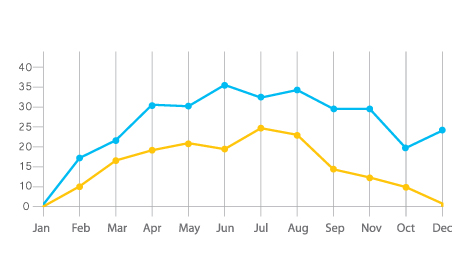
\includegraphics[scale=.6]{pic/graph_acc.jpg}
      \caption[กราฟแสดงความแม่นยำของการระบุตัวตนในแต่ละวัน]{กราฟแสดงความแม่นยำของการระบุตัวตนในแต่ละวัน}
      \label{fig:face_graph}
    \end{center}
  \end{figure}

\indent จากกราฟจะเห็นได้ว่าความแม่นยำเมื่อเวลาในการจัดเก็บข้อมูลนั้นมากขึ้นก็จะทำให้ความแม่นยำสูงขึ้น แต่จะมีจุดที่ความแม่นยำสูงที่สุดและลดลงเรื่อยเนื่องจาก
ข้อมูลรูปภาพใบหน้ามีจำนวนที่เกินไปทำให้ความแม่นยำนั้นจะไม่สูงไปกว่าจัดนี้อีกแล้ว

\section{เวลาในการประมวลผลรูปภาพใบหน้า}
การทดสอบต่อไปนี้เป็นการทดสอบเพื่อวัดผลว่าเวลาในการประมวลผลรูปภาพใบหน้าตลอดจนระบุตัวตนที่ออกแบบนั้น
มีเวลาาที่มากหรือน้อยเพียงใดจากการบันทึกผลที่ Raspberry Pi โดยจะเปรียบเทียบที่วัดได้ในครั้งที่มีการตรวจจับภาพใบหน้า
เปรียบเทียบออกมาเป็นกราฟเส้นดังนี้
  
\begin{figure}[!ht]
  \begin{center}
    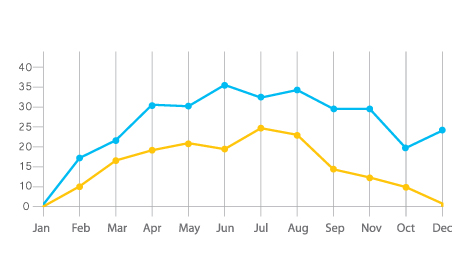
\includegraphics[scale=.7]{pic/graph_acc.jpg}
    \caption[กราฟแสดงเวลาในการประมวลผลของระบบในแต่ละวัน]{กราฟแสดงเวลาในการประมวลผลของระบบในแต่ละวัน}
    \label{fig:time_graph}
  \end{center}
\end{figure}
\newpage
\indent จากกราฟจะเห็นได้ว่าเวลาในการประมวลผลรูปภาพใบหน้า ส่งรูปภาพไปยังเซิร์ฟเวอร์ การระบุตัวตน และการส่งผลลัพธ์กลับมาแสดงผลในหน้าจอนั้นมีเวลาเฉลี่ย .... มิลลิวินาที



\section{ความพึงพอใจของการทดลอง}
จากการทดลองที่ห้องวิจัย OASYS ได้ทำการบันทึกผลความพึงพอใจของผู้ทดลองต่อระบบระบุตัวตนด้วยรูปภาพใบหน้าบุคคลที่ โดยจะได้ผลสรุปดังนี้

\begin{figure}[!ht]
    \begin{center}
      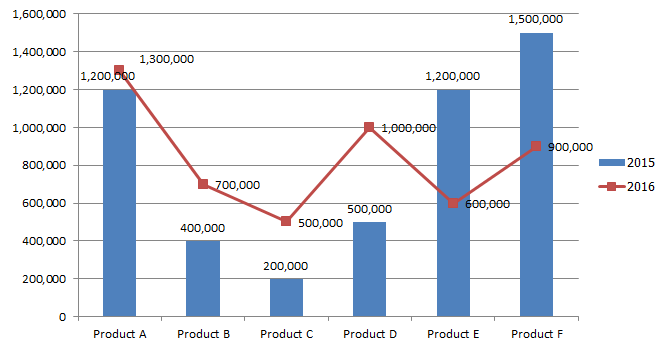
\includegraphics[scale=.5]{pic/bar_graph.png}
      \caption[กราฟแสดงความพึงพอใจของผู้ทดลอง]{กราฟแสดงความพึงพอใจของผู้ทดลอง}
      \label{fig:bar_graph}
    \end{center}
  \end{figure}